Also known as the adjoint state method, it is another example of a discrete method that aims to find the gradient by solving an alternative system of linear equations, known as the \textit{adjoint equations}, simultaneously with the original system of equations defined by the numerical solver. 
These methods are extremely popular in optimal control theory in fluid dynamics, for example for the design of geometries for vehicles and airplanes that optimize performance \cite{Elliott_Peraire_1996, Giles_Pierce_2000}.

The idea of the adjoint method is to treat the differential equation as a constraint in an optimization problem and then differentiate an objective function subject to that constraint. 
Mathematically speaking, this can be treated both from a duality or Lagrangian perspective \cite{Giles_Pierce_2000}.
In agreement with other authors, we prefer to derive the equation using the former as it may give better insights to how the method works and it allows generalization to other user cases \cite{Givoli_2021}. 
The derivation of adjoint methods using the Lagrangian formulation can be found in Appendix \ref{appendix:lagrangian}.
% Mathematically, reverse mode AD is related to the adjoint differential equations \cite{Griewack-on-AD}

% \subsubsection{Discrete differential equation}
\subsubsection{Adjoint state equations}

% reference: Sensitivity theory of non-linear systems

The derivation of the discrete adjoint equations is carried out once the numerical scheme for solving Equation \eqref{eq:original_ODE} has been specified.  
Given a discrete sequence of timesteps $t_0, t_1, \ldots, t_N$, we aim to find approximate numerical solutions $u_i \approx u(t_i; \theta)$. 
Any numerical solver, including the ones discussed in Section \ref{section:intro-numerical-solvers}, can be understood as solving the (in general nonlinear) system of equations defined by $G(U; \theta) = 0$, where $U$ is the super-vector $U = (u_1, u_2, \ldots, u_N) \in \R^{nN}$, and we had combine the systems of equations defined by the iterative solver as $G(U; \theta) = (g_1(u_1; \theta), \ldots, g_N(u_N; \theta)) = 0$ (see Equation \eqref{eq:solver-constriant-example}).

We are interested in differentiating an objective or loss function $L(U, \theta)$ with respect to the parameter $\theta$. 
Since here $U$ is the discrete set of evaluations of the solver, examples of loss functions now include 
\begin{equation}
    L(U, \theta) 
    = 
    \frac{1}{2} \sum_{i=1}^N \| u_i - u_i^\text{obs} \|^2, 
\end{equation}
with $u_i^\text{obs}$ the observed time-series. 
Now, same as Equation \eqref{eq:dLdtheta_VJP} we have 
\begin{equation}
    \frac{dL}{d\theta} 
    = 
    \frac{\partial L}{\partial \theta} 
    + 
    \frac{\partial L}{\partial U} \frac{\partial U}{\partial \theta}.
    \label{eq:dhdtheta0}
\end{equation}
We further need to impose the constraint that the solution satisfies the algebraic equation $G(U; \theta) = 0$, which gives
\begin{equation}
    \frac{dG}{d\theta} 
    = 
    \frac{\partial G}{\partial \theta} 
    + 
    \frac{\partial G}{\partial U} \frac{\partial U}{\partial \theta}
    =
    0
\end{equation}
and which is equivalent to 
\begin{equation}
    \frac{\partial U}{\partial \theta} 
    = 
    - \left( \frac{\partial G}{\partial U} \right)^{-1} \frac{\partial G}{\partial \theta}.
\end{equation}
If we replace this last expression into equation \eqref{eq:dhdtheta0}, we obtain
\begin{equation}
    \frac{dL}{d\theta} 
    =
    \frac{\partial L}{\partial \theta} 
    - 
    \frac{\partial L}{\partial U}
    \left( \frac{\partial G}{\partial U} \right)^{-1} 
    \frac{\partial G}{\partial \theta}.
    \label{eq:dhdtheta}
\end{equation}
The important trick in the adjoint state methods is to observe that in this last equation, the right-hand side can be resolved as a vector-Jacobian product (VJP), with $\frac{\partial L}{\partial U}$ being the vector.
Instead of computing the product of the matrices $\left( \frac{\partial G}{\partial U} \right)^{-1}$ and $\frac{\partial G}{\partial \theta}$, it is computationally more efficient first to compute the resulting vector from the VJP operation $\frac{\partial L}{\partial U} \left( \frac{\partial G}{\partial U} \right)^{-1}$ and then multiply this by $\frac{\partial G}{\partial \theta}$.
This leads to the definition of the adjoint $\lambda \in \R^{nN}$ as the solution of the linear system of equations 
\begin{equation}
    \left( \frac{\partial G}{\partial U}\right)^T \lambda 
    =  
    \left( \frac{\partial L}{\partial U} \right)^T,
    \label{eq:adjoint-state-equation}
\end{equation}
or equivalently,
\begin{equation}
    \lambda^T = \frac{\partial L}{\partial U} \left( \frac{\partial G}{\partial U} \right)^{-1}.
    \label{eq:def_adjoint}
\end{equation}
Finally, if we replace Equation \eqref{eq:def_adjoint} into \eqref{eq:dhdtheta}, we obtain 
\begin{equation}
    \frac{dL}{d\theta} 
    =
    \frac{\partial L}{\partial \theta} 
    - 
    \lambda^T \frac{\partial G}{\partial \theta}.
    \label{eq:gradient-adjoint-state-method}
\end{equation}
The important trick used in the adjoint method is the rearrangement of the multiplicative terms involved in equation \eqref{eq:dhdtheta}. 
Computing the full Jacobian/sensitivity $\partial U / \partial \theta$ will be computationally expensive and involves the product of two matrices. 
However, we are not interested in the calculation of the Jacobian, but instead in the VJP given by $\frac{\partial L}{\partial U} \frac{\partial U}{\partial \theta}$. 
By rearranging these terms and relying in the intermediate variable $G(U; \theta)$, we can make the same computation more efficient. 
These ideas are summarized in the diagram in Figure \ref{fig:discrete-adjoint}, where we can also see an interesting interpretation of the adjoint as being equivalent to $\lambda^T = - \frac{\partial L}{\partial G}$. 

\begin{figure}[t]
    \centering
    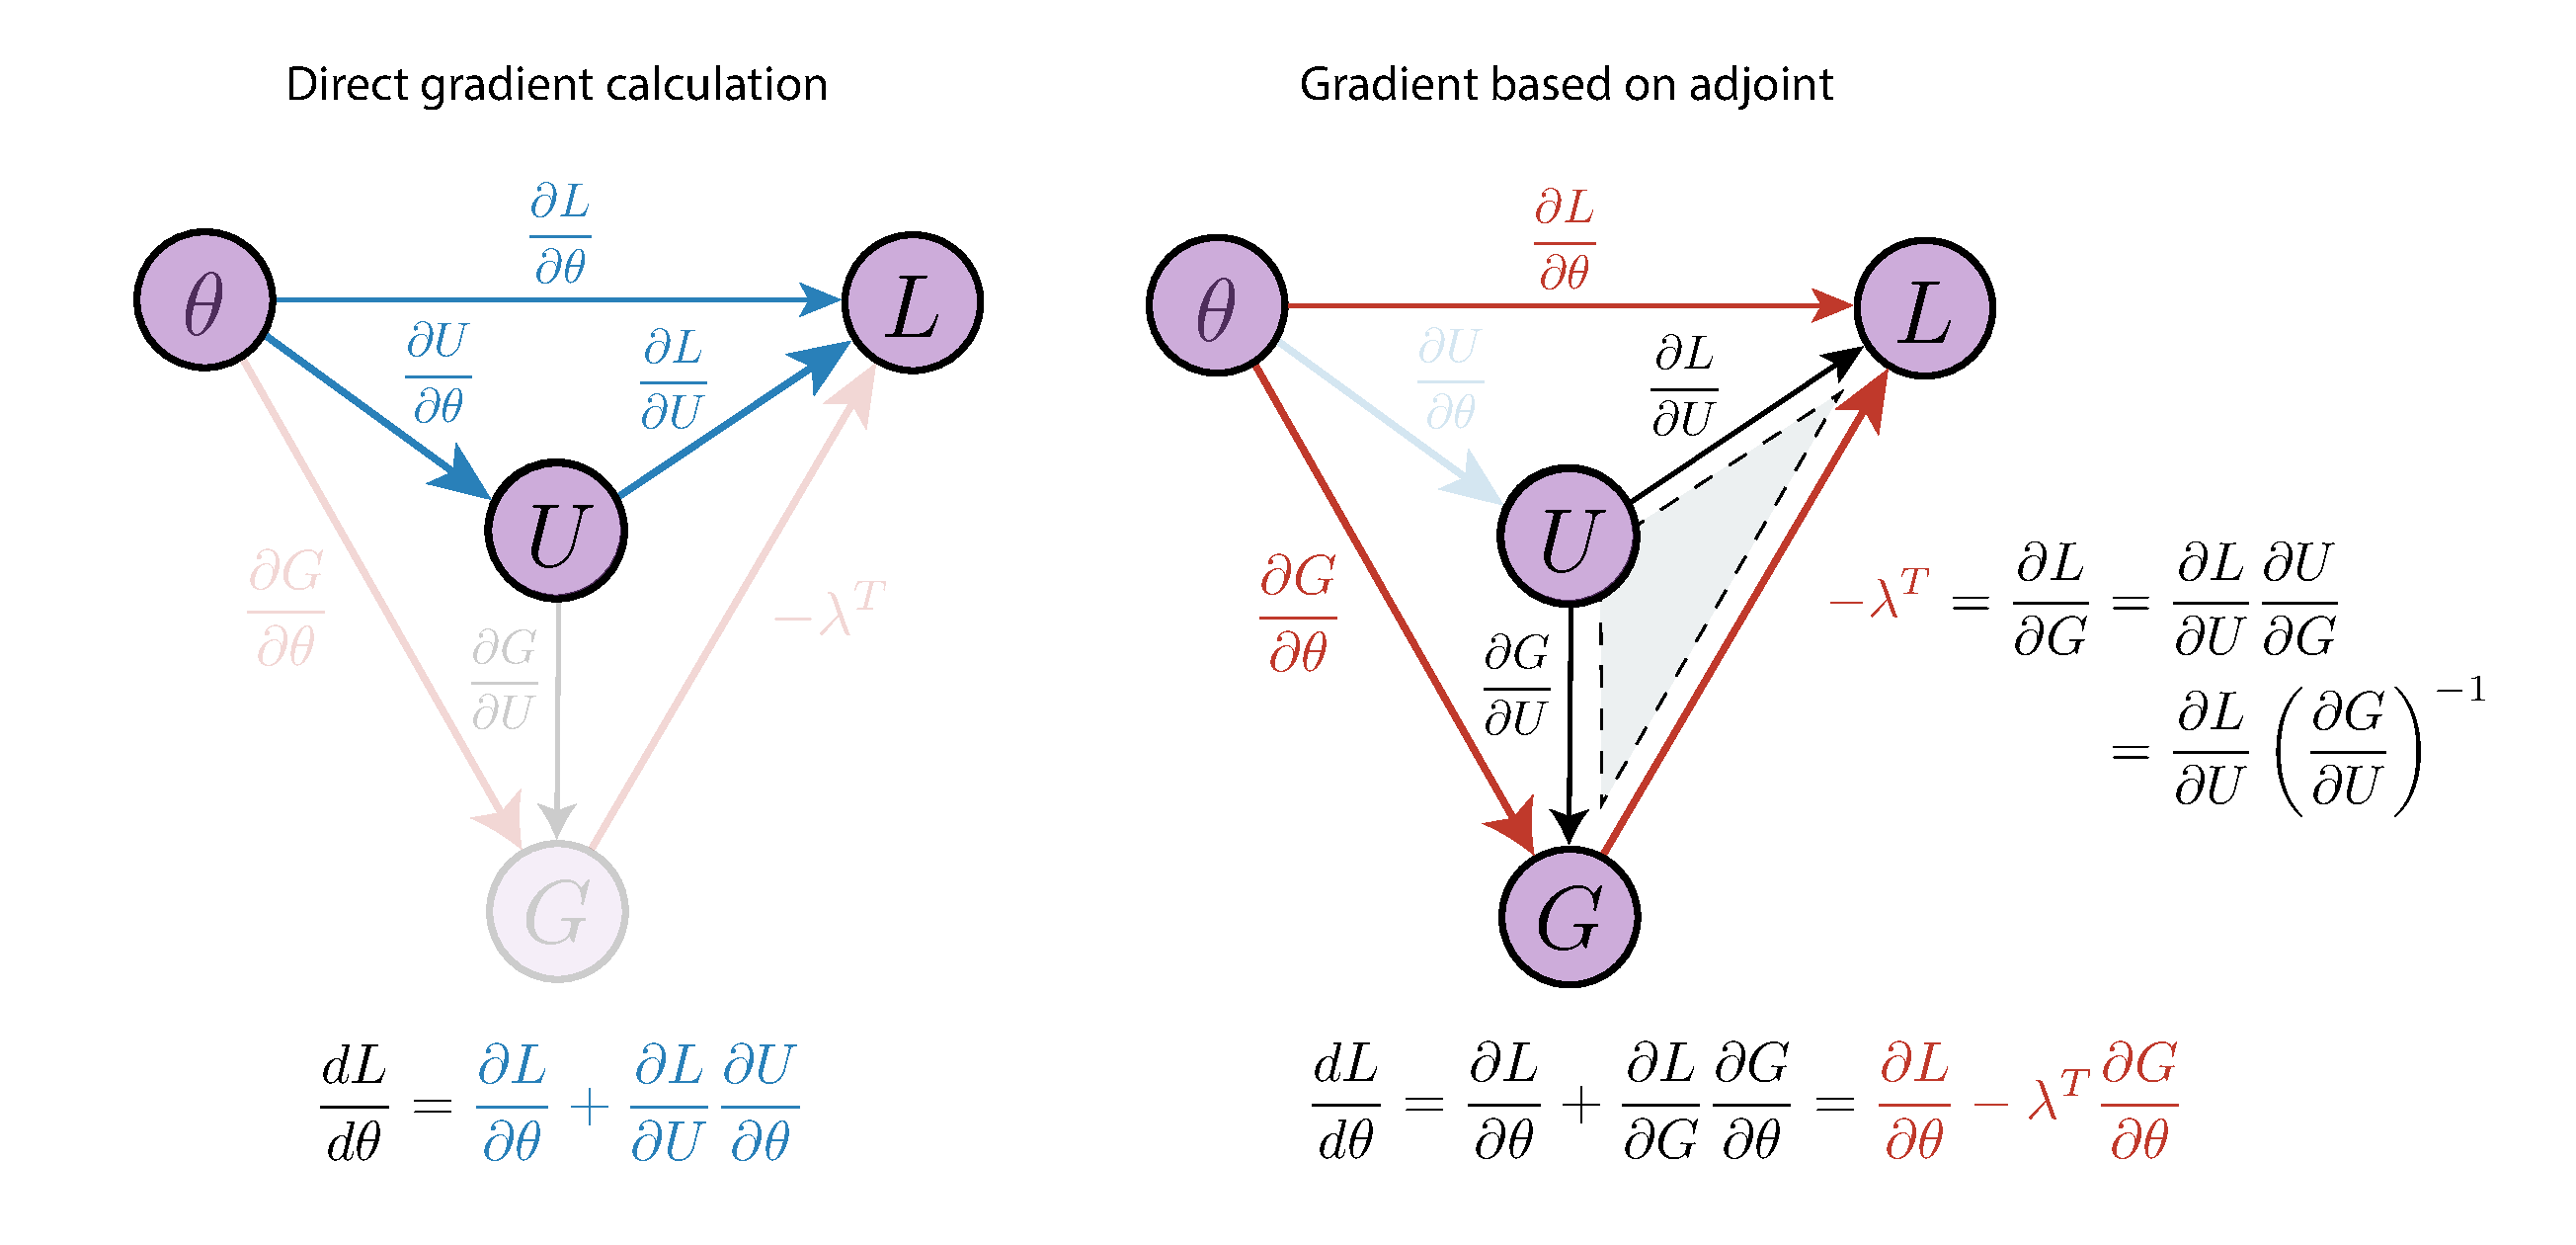
\includegraphics[width=0.95\textwidth]{figures/discrete_adjoint.pdf}
    \caption{Diagram showing how gradients are computed using discrete adjoints. On the left, we see how gradients will be computed if we use the chain rule applied to the directed triangle defined by the variables $\theta$, $U$, and $L$ (blue arrows). However, we can define the intermediate vector variable $G = G(U; \theta)$, which satisfies $G  = 0$ as long as the discrete system of differential equations are satisfied, and apply the chain rule instead to the triangle defined by $\theta$, $G$, and $L$ (red arrows). In the red diagram, the calculation of $\frac{\partial L}{\partial G}$ is done by pivoting in $U$ as shown in the right diagram (shaded area). Notice that the use of adjoints avoids the calculation of the sensitivity $\frac{\partial U}{\partial \theta}$. The adjoint is defined as the partial derivative $\lambda^T = - \frac{\partial L}{\partial G}$ representing changes in the loss function due to variations in the discrete equation $G(U; \theta) = 0$. 
    }
    \label{fig:discrete-adjoint}
\end{figure}


Notice that the algebraic equation of the adjoint $\lambda$ in Equation \eqref{eq:adjoint-state-equation} is a linear system of equations even when the original system $G(U; \theta)=0$ was not necessarily linear in $U$.
This means that while the forward mode may require multiple iterations in order to solve the non-linear system $G(U) = 0$ (e.g., by using Krylov methods), the backwards step to compute the adjoint is one single linear system of equations. 

\subsubsection{Simple linear system}

To gain further intuition about the discrete adjoint method, let us consider the simple case of the explicit linear one-step methods, where at every step we need to solve the equation $u_{i+1} = g_i (u_i; \theta) = A_i (\theta) \, u_i + b_i(\theta)$, where $A_i(\theta) \in \R^{n \times n}$ and $b_i(\theta) \in \R^n$ are defined by the numerical solver \cite{Johnson}. 
This condition can be written in a more compact manner as $G(U)=A(\theta) U - b(\theta) = 0$, that is 
\begin{equation}
    A(\theta) U 
    = 
    \begin{bmatrix}
        \I_{n \times n} & 0 &   &  & \\
        -A_1 & \I_{n \times n} & 0 &  &  \\
          & -A_2 & \I_{n \times n} & 0 &  \\
         &  &   & \ddots &   \\
         &  &  & -A_{N-1} & \I_{n \times n}
    \end{bmatrix}
    \begin{bmatrix}
        u_1 \\
        u_2 \\
        u_3 \\
        \vdots \\
        u_N
    \end{bmatrix}
    = 
    \begin{bmatrix}
        A_0 u_0 + b_0 \\
        b_1 \\
        b_2 \\
        \vdots \\
        b_{N-1}
    \end{bmatrix}
    = 
    b(\theta), 
\end{equation}
with $\I_{n \times n}$ the identity matrix of size $n \times n$.
% It is usually convenient to write this system of linear equations in the residual form $G(U; \theta) = 0$, where $G(U; \theta) = A(\theta) U - b(\theta)$ is the residual between both sides of the equation. 
% Different numerical schemes will lead to different design matrix $A(\theta)$ and vector $b(\theta)$, but ultimately every numerical method will lead to a system of linear equations with the form $G(U; \theta) = A(\theta) U - b(\theta) = 0$ after being discretized. 
Notice that in most cases, the matrix $A(\theta)$ is quite large and mostly sparse. 
While this representation of the discrete differential equation is  convenient for mathematical manipulations, when solving the system we rely on iterative solvers that save memory and computation. 

For the linear system of discrete equations $G(U; \theta)=A(\theta) U - b(\theta)=0$, we have 
\begin{equation}
    \frac{\partial G}{\partial \theta} 
    = 
    \frac{\partial A }{\partial \theta} U - \frac{\partial b}{\partial \theta},
\end{equation}
so the desired gradient in Equation \eqref{eq:gradient-adjoint-state-method} can be computed as 
\begin{equation}
    \frac{dL}{d\theta} 
    = 
    \frac{\partial L}{\partial \theta} 
    - 
    \lambda^T \left( \frac{\partial A }{\partial \theta} U - \frac{\partial b}{\partial \theta} \right)
    \label{eq:dhdtheta_linear}
\end{equation}
with $\lambda$ the discrete adjoint obtained by solving the linear system in Equation \eqref{eq:adjoint-state-equation},
\begin{equation}
    A(\theta)^T \lambda 
    =
    \begin{bmatrix}
        \I_{n \times n} & -A_1^T &   &  & \\
        0 & \I_{n \times n} & -A_2^T &  &  \\
          & 0 & \I_{n \times n} & -A_3^T &  \\
         &  &   & \ddots & -A_{N-1}^T  \\
         &  &  & 0 & \I_{n \times n}
    \end{bmatrix}
    \begin{bmatrix}
        \lambda_1 \\
        \lambda_2 \\
        \lambda_3 \\
        \vdots \\
        \lambda_N
    \end{bmatrix}
    = 
    \begin{bmatrix}
        u_1 - u_1^\text{obs} \\
        u_2 - u_2^\text{obs} \\
        u_3 - u_3^\text{obs} \\
        \vdots \\
        u_N - u_N^\text{obs}     
    \end{bmatrix}
    = 
    \frac{\partial L}{\partial U}^T.
    \label{eq:linea-adjoint-state-equation}
\end{equation}
This is a linear system of equations with the same size of the original $A(\theta) U = b(\theta)$, but involving the adjoint matrix $A^T$. 
Computationally this also means that if we can solve the original system of discretized equations then we can also solve the adjoint at the same computational cost (e.g., by using the LU factorization of $A(\theta)$). 
% One way of doing this is relying on matrix factorization. 
% Using the LU factorization we can write the matrix $A(\theta)$ as the product of a lower and upper triangular matrix, $A (\theta) = LU$, which then can be used for solving the adjoint equation since $A^T(\theta)=U^TL^T$.
Another more natural way of finding the adjoints $\lambda$ is by noticing that the system of equations \eqref{eq:linea-adjoint-state-equation} is equivalent to the final value problem 
\begin{equation}
    \lambda_{i} = A_{i}^T \lambda_{i+1} + (u_i - u_i^\text{obs})
    \label{eq:adjoint-discrete-linear-example}
\end{equation}
with final condition $\lambda_N$. 
This means that we can solve the adjoint equation backwards, i.e., in reverse mode, starting from the final state $\lambda_N$ and computing the values of $\lambda_i$ in decreasing index order. 
Unless the loss function $L$ is linear in $U$, this procedure requires to know the value of $u_i$ (or some equivalent form of it) at any given timestep. 